\documentclass[xcolor={dvipsnames}]{beamer}

\usetheme{Malmoe}
\usecolortheme{seagull}
\usepackage[]{natbib}
\usepackage{textpos}
\usepackage{amsmath, amssymb, bm}
\usepackage{multirow}
\usepackage{framed}
\usepackage{schemata}
\setbeamertemplate{navigation symbols}{}
\usepackage[english]{babel}
\usepackage{animate}
\usepackage{graphics}
\usepackage{fontawesome}


\definecolor{lightblue}{rgb}{0.145,0.6666,1} % Defines the color used for content box headers
\definecolor{Red}{rgb}{0.9,0.15,0}
\definecolor{Blue}{RGB}{55,126,184}
\definecolor{Green}{RGB}{77,175,74}
\definecolor{White}{RGB}{255,255,255}
\definecolor{Lightgray}{rgb}{0.86,0.86,0.86}

\setbeamertemplate{footline}
{
	\leavevmode%
	\hbox{%
		\begin{beamercolorbox}[wd=.50\paperwidth,ht=2.25ex,dp=1ex,center]{author in head/foot}%
			\usebeamerfont{author in head/foot}\insertshortauthor%% \beamer@ifempty{\insertshortinstitute}{}{(\insertshortinstitute)}
		\end{beamercolorbox}%
%		\hskip2pt%
		\begin{beamercolorbox}[wd=.50\paperwidth,ht=2.25ex,dp=1ex,center]{title in head/foot}%
			\usebeamerfont{title in head/foot}\insertshorttitle~~~~~~~~~~~~~~~~~~~~~~~~~~\insertframenumber
		\end{beamercolorbox}%
	}%
	\vskip0pt%
}
\makeatother

\title[Lifespan variation in Mexico]{
	\small{\textsl{BSPS 2017}}\\$\,$\\$\,$}

\subtitle{\large{\textsc{Homicide increase variation in lifespans in Mexico and its states}}\\$\,$\\}


\author[BSPS. Aburto \& Beltr\'an-S\'anchez 2017]
{
	\vspace{-0.5cm}
	\texorpdfstring{
		\begin{columns}
			\column{.9\linewidth}
			\centering
			\normalsize{Jos\'{e} Manuel Aburto}\\
			$\,$\\
			
\includegraphics[scale=0.2]{Figures/logos.png}     
		\end{columns}
	}
	{Jos\'{e} Manuel Aburto}
}

\date[]{ September 7 2017}

\beamertemplatenavigationsymbolsempty
\begin{document}


\begin{frame}[plain]
	\titlepage
\end{frame}
%%%%%%%%%%%%%%%%%%%%%%%%%%%%%%%%%%%%%%%%%%%%%%%%%%%%%%%%%%%%%%%%%%%%%%%%%
%%%%%%%%%%%%%%%%%%%%%%%%%%%%%%%%%%%%%%%%%%%%%%%%%%%%%%%%%%%%%%%%%%%%%%%%%
\section{Introduction}

%%%%%%%%%%%%%%%%%%%%%%%%%%%%%%%%%%%%%%%%%%%%%%%%%%%%%%%%%%%%%%%%%%%%%%%%%
\begin{frame}
\Large{
		\begin{itemize}
		
		\item<1-> \textbf{Violence} is main public health issue in Latin America.
		
		\item<2-> This region has the \textbf{highest} homicide rate in the world (16.3 per 100,000).
		
        \item<3-> Central American countries $\longrightarrow$ \textbf{upsurge} in homicides in the new century.

        \item<4-> \textbf{In Mexico, rates doubled between 2007 and 2012} (9.3 $\longrightarrow$ 18.6).
		
		\end{itemize}
		
}

\end{frame}


\begin{frame}\frametitle{As a result}

\Large{
		\begin{itemize}
		    
		\item Male life expectancy \textbf{stagnated} in the first decade of the 2000's ($\backsim $72y)
		
				\end{itemize}
		
		\pause
				\begin{center}
		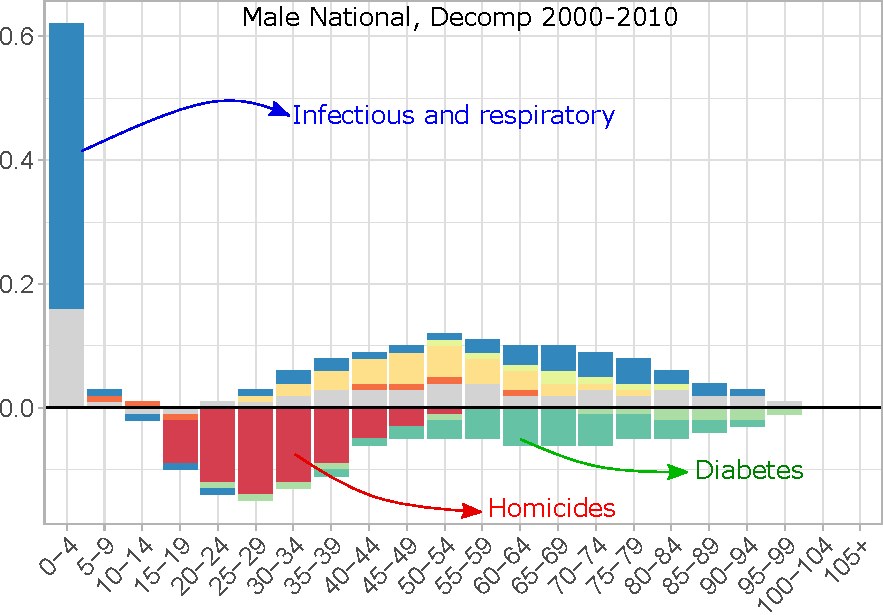
\includegraphics[scale=.55]{Figures/Fig_1}
				\end{center}
				

}
\end{frame}

\begin{frame}

\begin{center}
		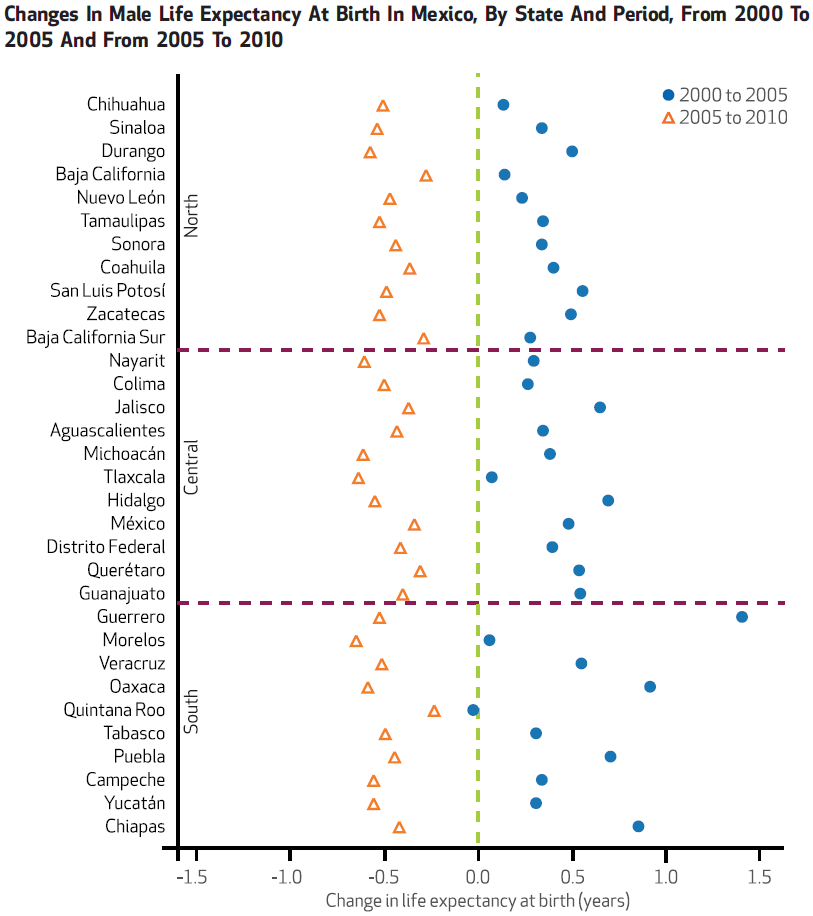
\includegraphics[scale=.423]{Figures/State_changes_e0}
				\end{center}			
		

\end{frame}



\begin{frame}\frametitle{Why lifespan variation?}
\Large{
		\begin{itemize}
		
		\item<1-> $e_0$ \textbf{conceals} variation of lifespans.

		\item<2-> We make decisions based on \textbf{both}.
		
		\item<3-> Expresses a \textbf{fundamental inequality}.
		
		\item<4-> Homicides affect mainly \textbf{young men}.
						
		\end{itemize}

}
\end{frame}

\section{Methods}

\begin{frame}\frametitle{Classification of deaths}
\large{
\begin{center} We use the concept of \textbf{``Avoidable/Amenable"} mortality. \end{center}
%An approach to approximate the impact of healthcare and other interventions, and to reveal potential areas of improvement. Based on causes that should not occur in the presence of effective and timely healthcare.
		\begin{enumerate}
		
		
\color{blue} 		\item Amenable to medical intervention \begin{tiny}Infectious \& respiratory, birth conditions\end{tiny}

\pause

\color{ForestGreen}		\item Diabetes
		
		\item Ischemic heart diseases (IHD)
		
		\item Lung cancer.
		 
		\item Cirrhosis.
		
\pause
		
\color{red}		\item Homicide
		
		\item Road traffic accidents
		
		\pause
		
\color{gray}				\item Rest.

		
		\end{enumerate}			

}
\end{frame}


\begin{frame}

\Large{
$e^{\dagger}\longrightarrow  $ average remaining life expectancy when death occurs.

\begin{itemize}
\item Easy \textbf{public health interpretation}.
\pause
\item Quantify age and cause specific effect in $e^{\dagger}$.
\pause
\item Separate ages that \textbf{decrease} from those that \textbf{increase} $e^{\dagger}$.
\end{itemize}

}
\end{frame}


\section{Results}

\begin{frame}

\Large{
Remember the stagnation in 2000-10?

				\begin{center}
		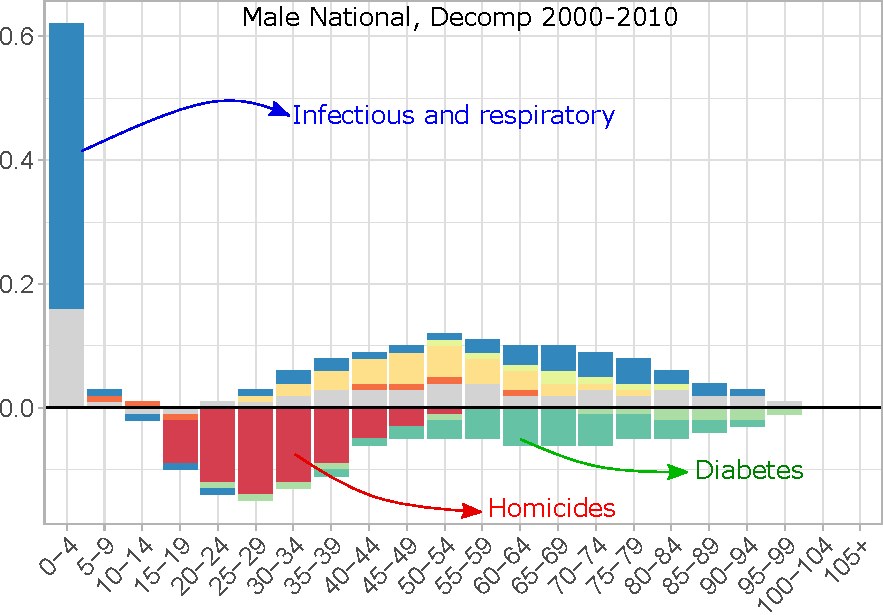
\includegraphics[scale=.65]{Figures/Fig_1}
				\end{center}
				

}
\end{frame}


\begin{frame}

\Large{
Now $e^\dagger \backsim$ 15y

				\begin{center}
		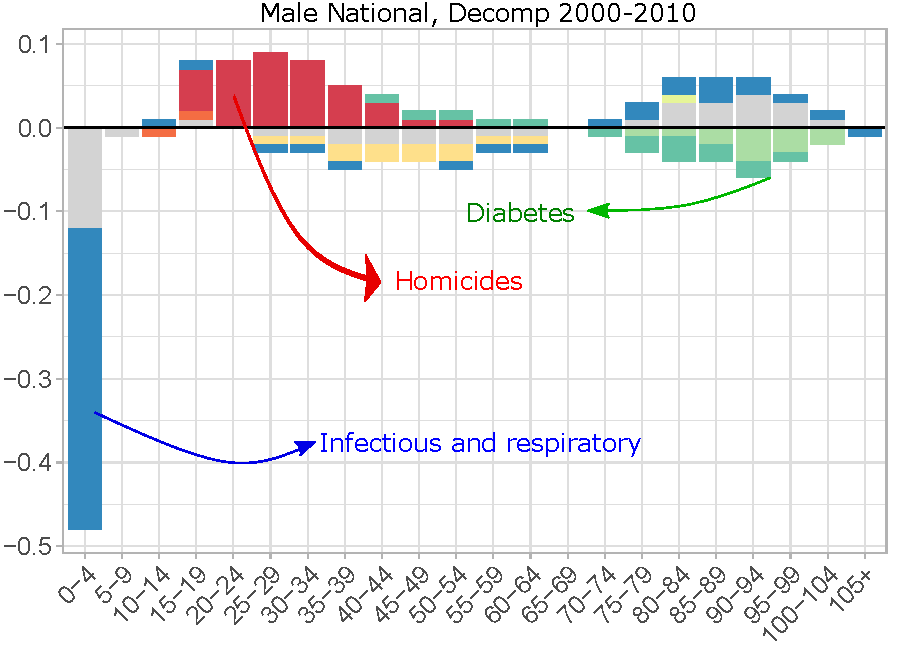
\includegraphics[scale=.65]{Figures/Cause_ed_decomp_Males}
				\end{center}				

}
\end{frame}


\begin{frame}

\Large{
Now rescale

				\begin{center}
		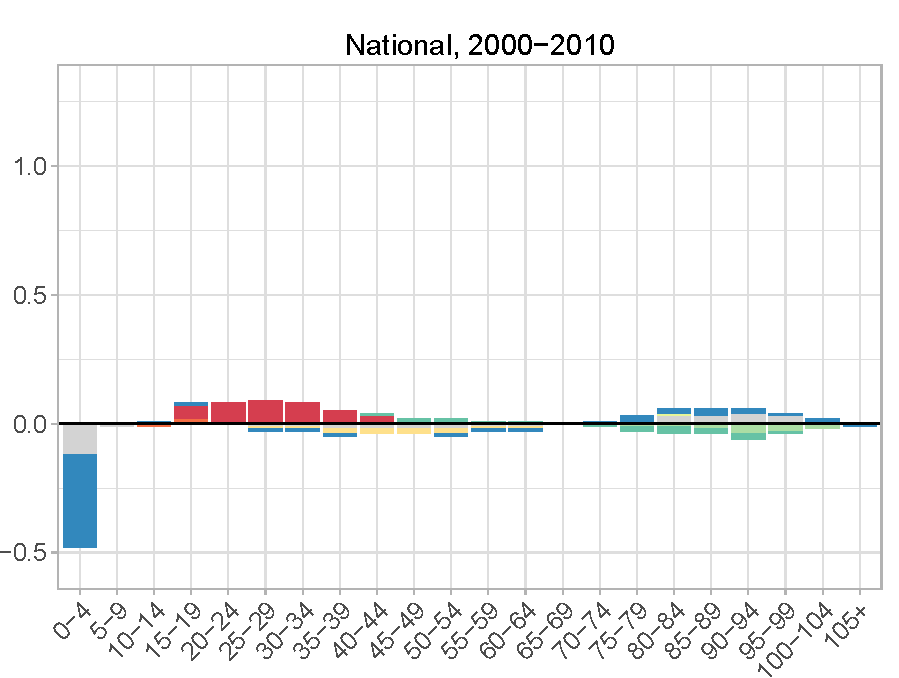
\includegraphics[scale=.65]{Figures/Cause_ed_decomp_Males2}
				\end{center}				

}
\end{frame}

\begin{frame}

\Large{
Now the most dangerous state in Mexico in 2010

				\begin{center}
		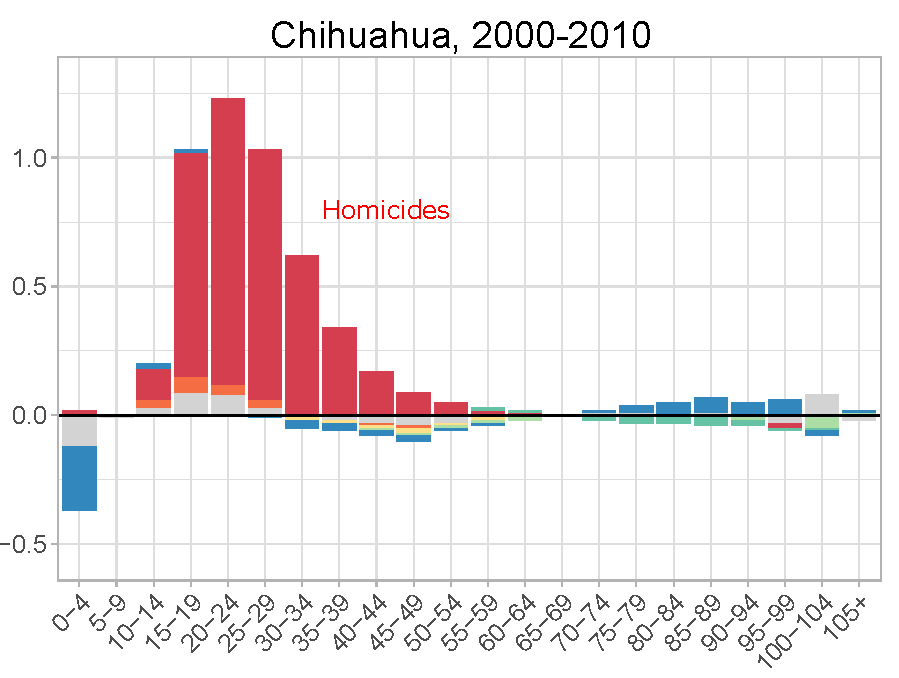
\includegraphics[scale=.65]{Figures/Cause_ed_decomp_Males_Chihuahua}
				\end{center}				

}
\end{frame}


\begin{frame}

\Large{
Rates 3 times of US troops in Iraq between 2003 and 2006!
				\begin{center}
		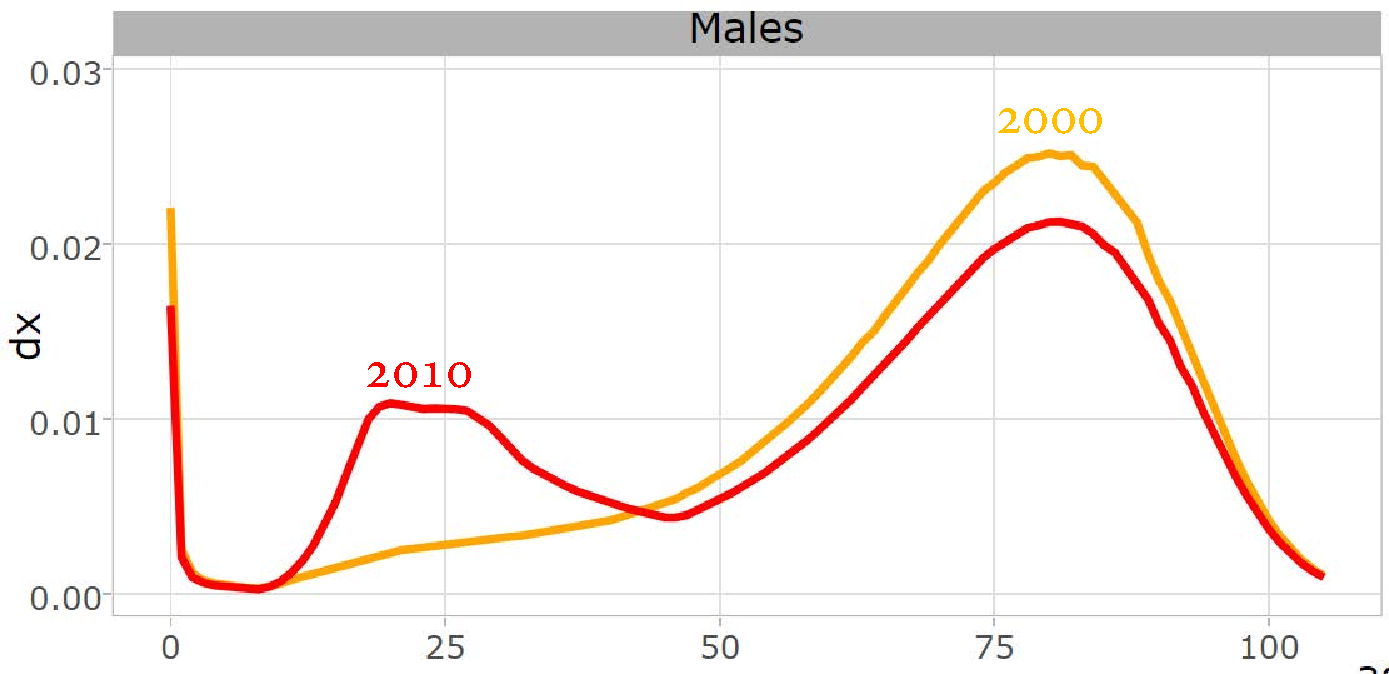
\includegraphics[scale=.45]{Figures/Distr_chihuahua}
				\end{center}				

}
\end{frame}



\begin{frame}

\Large{
Now in the last decade, 10y of War on drugs!!

				\begin{center}
		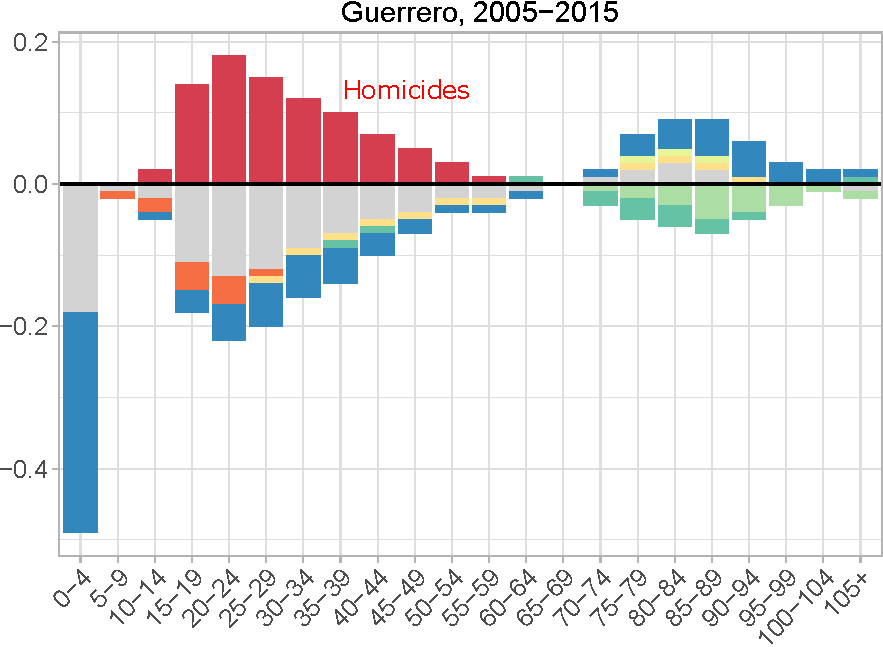
\includegraphics[scale=.65]{Figures/Cause_ed_decomp_Males_Guerrero}
				\end{center}				

}
\end{frame}

\begin{frame}

\Large{
2 of most dangerous cities in the world in 2016 in this state (The Economist)!

				\begin{center}
		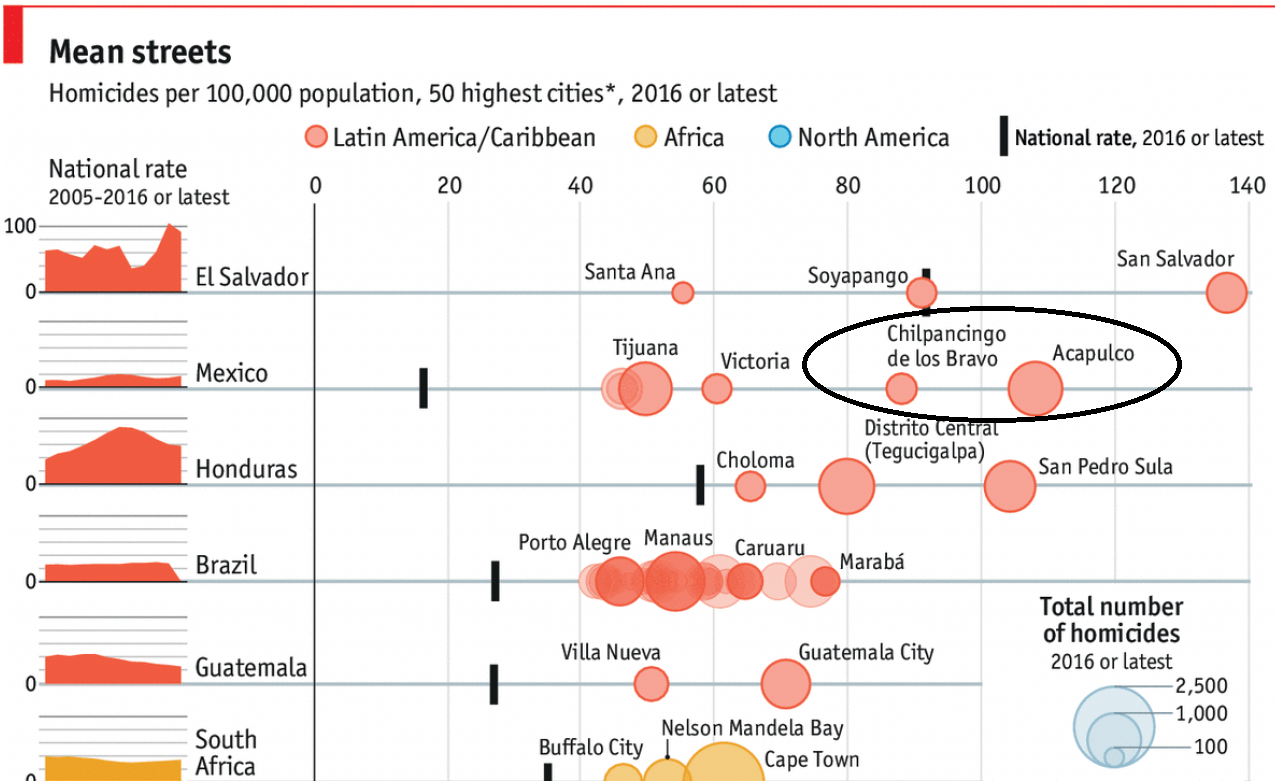
\includegraphics[scale=.38]{Figures/Capture}
				\end{center}				

}
\end{frame}

\begin{frame}

\Large{
10 years and still not recovered!

							\begin{center}		
\animategraphics[autoplay, scale=0.5]{3}{Figures/Cause_ed_decomp_Males_states}{1}{33}
				\end{center}
				

}
\end{frame}






%%%%%%%%%%%%%%%%%%%%%%%%%%%%%%%%%%%%%%%%%%%%%%%%%%%%%%%%%%%%%%%%%%%%%%%%

%%%%%%%%%%%%%%%%%%%%%%%%%%%%%%%%%%%%%%%%%%%%%%%%%%%%%%%%%%%%%%%%%%%%%%%%
\begin{frame}
 \begin{center}
	\begin{center}
	 \textbf{Challenge of Mexico: reduce violence}
	\end{center}
	
	\bigskip
	\bigskip
More information: 

Email: jmaburto@health.sdu.dk 

\faTwitter \quad  @jm\_aburto 

\faGithub \quad @jmaburto 

Shinnyapp: \url{<https://jmaburto.shinyapps.io/LVMx_App/>}


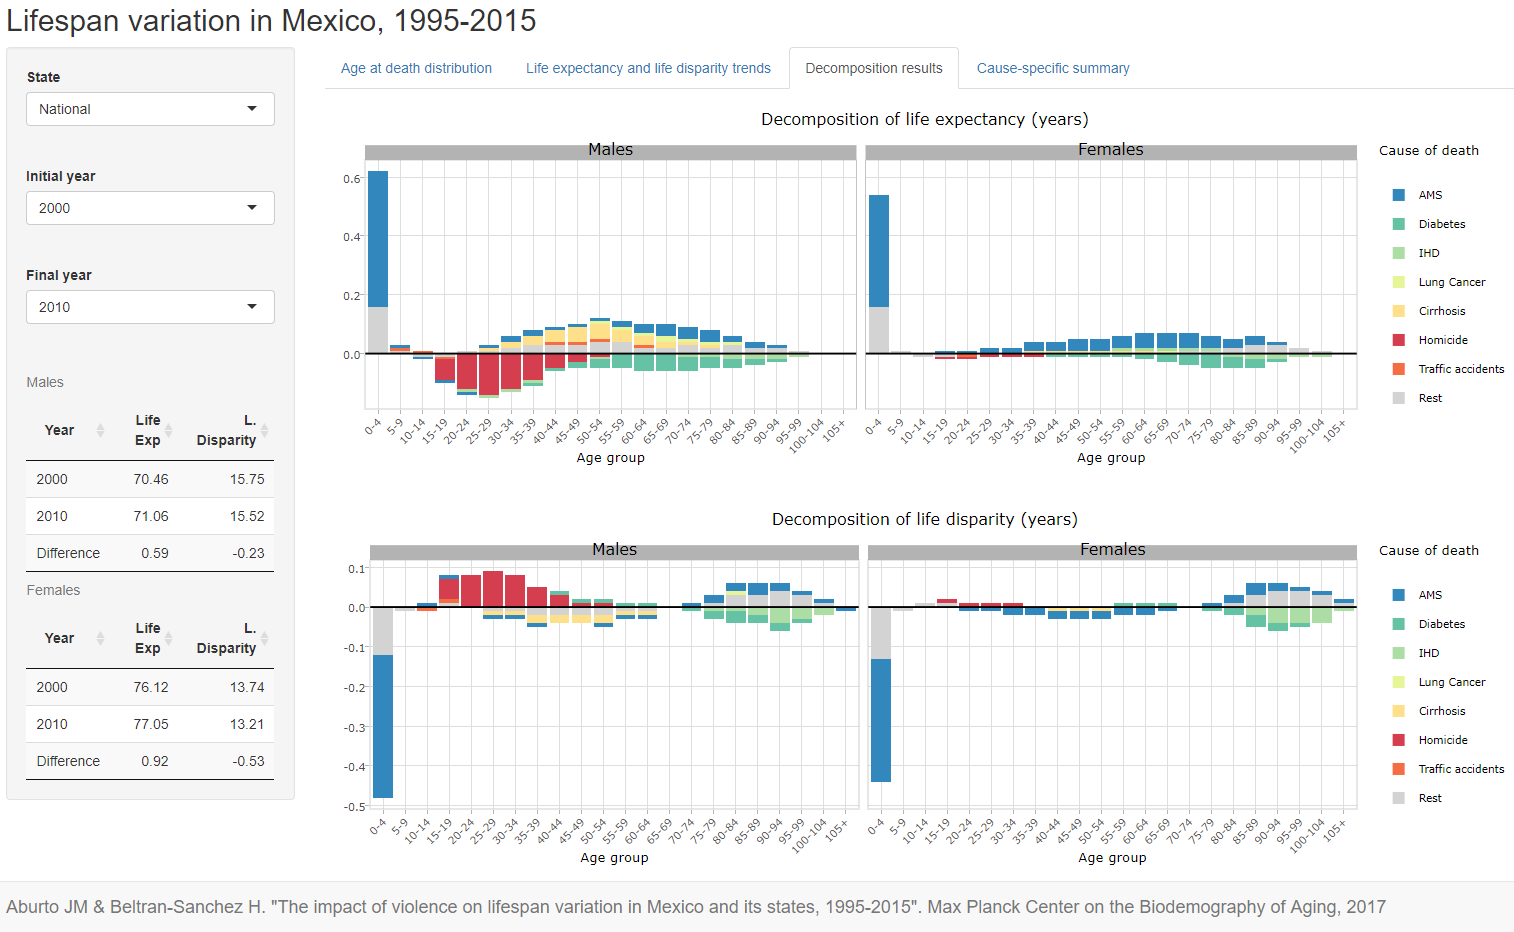
\includegraphics[scale=0.23]{Figures/Shinnyapp_fig} \\   

 

\end{center}
 
 

\end{frame}



\end{document}
	

